\begin{frame}
\frametitle{WP IDE} 
L'objectif du WP IDE est de construire une interface de programmation en Coq plus orientée vers l'aide à la programmation que l'actuel CoqIde.
%% L'AIDE À LA PROGRAMMATION ?
% non, pas "plus orientée vers l'aide" non plus. juste plus élaborée avec plus de fonctionalités, et moins de bug (mais pas pour l'instant)
\end{frame}

\begin{frame}
Ce que Coquille fait et que CoqIde ne fait pas au niveau du code :
\begin{itemize}
    \item Les numéros de ligne.
    \item Le code folding (replier des lignes de code en une seule, pour une preuve par exemple).
    \item Des raccourcis plus "classiques", et personnalisables.
    \item Possibilité de faire "Redo" après des "Undo".
\end{itemize}
\end{frame}

\begin{frame}

Au niveau du langage :
\begin{itemize}
    \item La gestion de Ltac Debug, avec une interface de parcours des résultatsScreenshot
    \item Plusieurs instances de Coqtop, une par onglet ouvert
    \item Un affichage des résultats au choix : classique ou LaTeX-likeScreenshot
    \item L'action "Next/Previous" d'envoi d'une commande est considérée comme une action comme les autres, donc "Undo/Redo" agit dessus
\end{itemize}
 
\end{frame}

\begin{frame}

Ce que CoqIde fait au niveau du code :

\begin{itemize}
    \item Lister les tactiques existantes dans un menu.
    \item Lister les actions disponibles par click droit sur une hypothèse ou un but.
\end{itemize}



\end{frame}


\begin{frame}

Au niveau du langage :

\begin{itemize}
    \item Le Proof Wizard.
%    \item La gestion des Write State / Restore State
    \item La gestion de l'aide.
    \item La gestions de la compilation.
\end{itemize}


\end{frame}



\begin{frame}
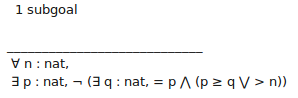
\includegraphics[width=1\textwidth]{../images/ide/unicode.png}
%ça ne compile pas ! Ajoutez les images, bordel --> ``attention, des images ont été oubliées'' est plus agréable à lire.
%montrer des choses que ne peut pas faire coquille (quoi ?)
\end{frame}

\begin{frame}
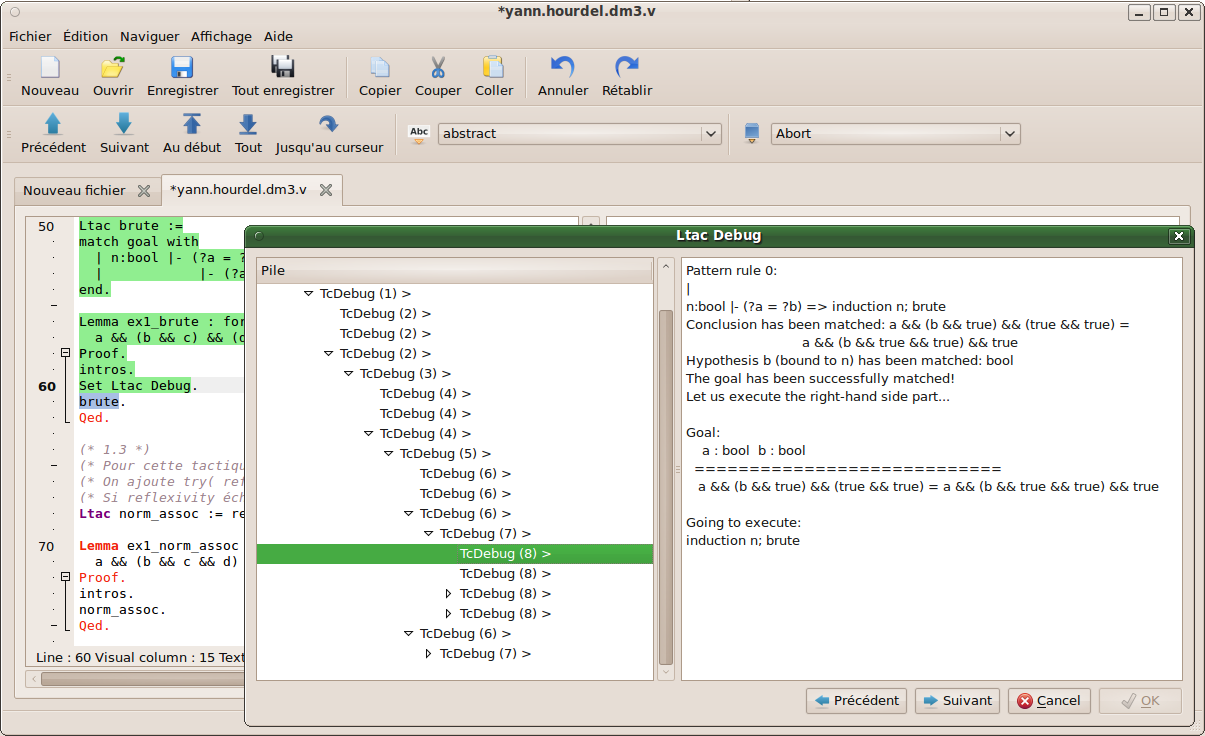
\includegraphics[width=1\textwidth]{../images/ide/ltacdebug.png}
%(ltac debug)
\end{frame}
